\section{MANO Benchmarking Framework} 

MANO Benchmarking Framework (MBF) is a result of a small script that was used to run the experiments discussed in the previous sections. The idea of MBF is to provide MANO developers with a generic framework for running experiments on MANO.
MBF mainly provides the following 1) Easy interfacing with MANO instances by using python-mano-wrappers, 2) Ability to run experiments with different service descriptors, 3) Collection of performance metrics in convenient data format and 4) Flexible graphing mechanism of the collected data. 


\subsection{Design}

MBF is designed for ease of use and low barrier to entry for developers. 
We explain the choice of tools that are used in MBF in the following list.

\begin{itemize}
	\item{\textbf{Netdata\footnote{https://github.com/netdata/netdata}}} is the metrics monitoring system for MBF. 
	Netdata captures relevant system metrics and provide powerful APIs to query the recorded data in a suitable format.
	\item{\textbf{Python}} as the choice of scripting language was obvious as the MANOs itself are implemented in python.
	\item{\textbf{python-mano-wrappers}} is used to provide access to REST APIs of MANOs from python.
	\item{\textbf{Docker}} is used to containerize MBF, thus making it easy to distribute and portable.
	\item{\textbf{Matplotlib}} is the graphing library for MBF due to its flexibility and ease of use.
	\item{\textbf{Flask}} as a python server that can be used to provide additional interactions with the experiment runner.

\end{itemize}


\subsection{Parameters and KPIs} 

\subsubsection{Parameters}

MBF has experiment parameters that can be altered. 
The following parameters are supported

\begin{itemize}
	\item{\textbf{Descriptors}} NSDs and VNFDs can be changed. 
	a list of NSDs/VNFDs is also supported. 
	When a list of descriptors are provided, the experiment will be run for each of the descriptors.
	\item{\textbf{Number of instances}} Total number of instantiation requests to be sent to the MANO.
	\item{\textbf{Number of runs}} number of re-runs of the same experiment to be run. 
	This is performed to measure the variance in results.
	\item{\textbf{Requests per minute (RPM)}} The rate at which the instantiation requests are sent to the MANO
	\item{\textbf{Observation Time}} The observation time after the instantiation requests are sent. 
	This can be used to collect metrics post instantiation to observe how MANO behaves in the monitoring phase.
	\item{\textbf{Inter-experiment Delay}} is the time between experiment runs. 
	This is altered to give enough time for the VIM to terminate and cleanup instances from the previous experiment runs if any.
	\item{\textbf{Skip experiment on error}} if set to true, the current run is skipped due to a failed instance on the VIM.

\end{itemize}

\subsection{Key Performance Indicators}

MBF stores resource utilization metrics during the experiment and generates graphs to visualize the results. 
However, these are only examples and the further possibilities are supported by the framework. 
The metrics are stored as CSV files.

\begin{itemize}
	\item{\textbf{CPU}} Overall system CPU usage is recorded as well as the individual docker micro service CPU usage metrics are stored.
	\item{\textbf{Memory}} Overall system memory usage along with the individual docker micro service memory usage is stored.
	\item{\textbf{System Load}} The 1m, 5m and 15m moving averages of system load values provided by the Linux kernel is stored.
	\item{\textbf{Status Tracking}} The status of all instances are stored by polling the VIM every 5 seconds over the experiment lifetime. 
	This enables to track the status change over time.
	\item{\textbf{End-to-end Deployment Time}} is the time elapsed to deploy all the instances on the VIM.
	\item{\textbf{Individual Deployment Time}} is the time taken by each instance for deployment. 
	This is also split into time taken by MANO and VIM.
\end{itemize}

\subsection{Steps for experiment run} 

The steps to run a basic experiment is detailed in this section. 
The following instruction is to run an experiment with 90 instances on OSM using an network service with 1 VNF. 

\begin{enumerate}
	\item Git clone the experiments-branch\footnote{https://github.com/CN-UPB/MANO-Benchmarking-Framework}
	\item Build and start the docker container
	\item Change experiment variables in the relevant scripts for respective MANOs
	\begin{itemize}
		\item \textbf{OSM} -- \textit{run-experiment-osm.py}
		\item \textbf{Sonata and Pishahang}  -- \textit{run-experiment-sonata.py}
		\item \textbf{Pishahang Container Orchestration} -- \textit{run-experiment-sonata-k8}
	\end{itemize}
	
	\item Run the relevant script from inside the container. 
	The experiment will now run and stores result files in the same directory
	\item Use the result parser from the \texttt{experiments/results/csv-result-parser.py} to parse the results and store it in a format suitable for graphing
	\item Use the graph plotter on the parsed files to generate the graphs\\ \texttt{experiments/results/plot-graphs.py}
	
	\end{enumerate}

The commands required to run these are listed in the readme file here, \\ \url{https://github.com/CN-UPB/MANO-Benchmarking-Framework/blob/master/README.md}

\textit{\\\textbf{Note:} This process is being streamlined to reduce some redundant steps and will be released in the next version of MBF.} 

\subsection{Example Use Cases}

In this section we demonstrate a few use cases of MBF. 
The framework facilitated easy experimentation, collection and analysis of metrics in the following cases. 
However, in-depth analysis of what the metrics and graphs mean are out of scope of this document. 



\subsubsection{Comparison of different network services} 

We compared the performance metrics of different NSDs/VNFDs and visualized it. 
For this, we provided 6 different network service descriptors to the experiment runner. 
First 3 NS consisted of a cirros image as a VNF with 1, 3 and 5 VNFs per NSD and the other 3 NS consisted of an Ubuntu image as a VNF with 1, 3 and 5 VNFs per NSD.\\

The experiment stores the KPIs listed in the previous section, along with the graphs visualizing the differences. 
This graph is produced for each micro-service showing the resource utilization of each NS under different number of instantiations. 
As an example, the figures \ref{fig:osmlcm-mean-cpu-cases} and \ref{fig:osmro-mean-cpu-cases} show the CPU utilization of the OSM microservice LCM and RO respectively.

\begin{figure}[h]
	\centering
	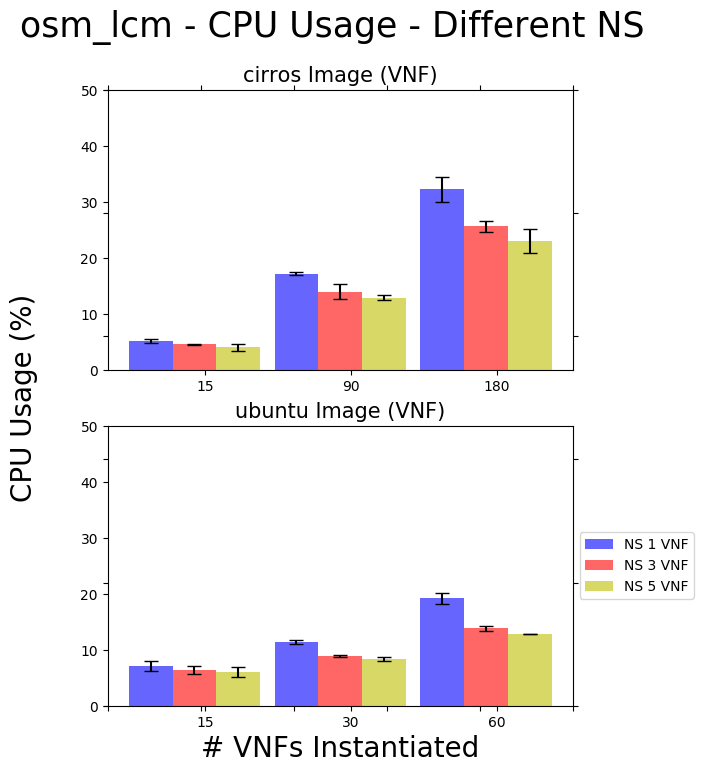
\includegraphics[width=0.6\linewidth]{figures/scalability_graphs/Docker-Grouped-Cases/osm/osm_lcm-Mean-CPU-Cases}
	\caption{CPU usage of OSM microservice LCM}
	\label{fig:osmlcm-mean-cpu-cases}
\end{figure}

\begin{figure}
	\centering
	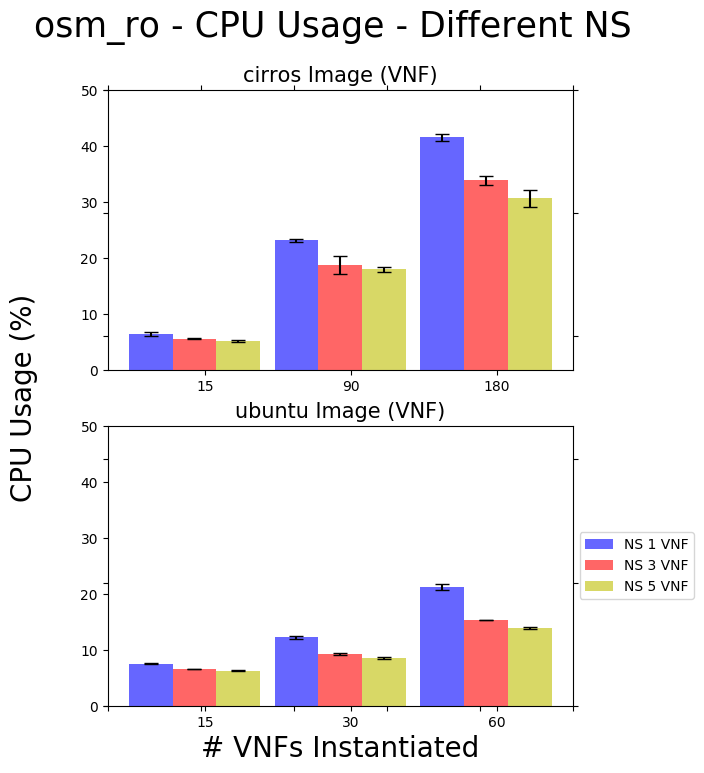
\includegraphics[width=0.6\linewidth]{figures/scalability_graphs/Docker-Grouped-Cases/osm/osm_ro-Mean-CPU-Cases}
	\caption{CPU usage of OSM microservice RO}
	\label{fig:osmro-mean-cpu-cases}
\end{figure}

\pagebreak

\subsubsection{Container vs VM Orchestration} 
\label{vmvscontainer}
Pishahang supports container orchestration on kubernetes and OSM supports VM orchestration on OpenStack. 
We compared the performance of orchestrating similar network services on VM and containers. 
In the figure \ref{fig:timecomparison}, the graph on top shows the average time distribution between MANO and VIM for deploying one network service with one VNF. 
The bottom graph in the figure \ref{fig:timecomparison} shows the total time taken to deploy 90 instances of a network with one VNF. 
The time taken to deploy similar VNFs is significantly less for containers, which is expected as containers are light weight compared to a VMs. \\

\textit{Note:} Pishahang support for VM orchestration is not stable, hence, we could not perform similar VM experiments on Pishahang for this comparison.

\begin{figure}[h]
	\centering
	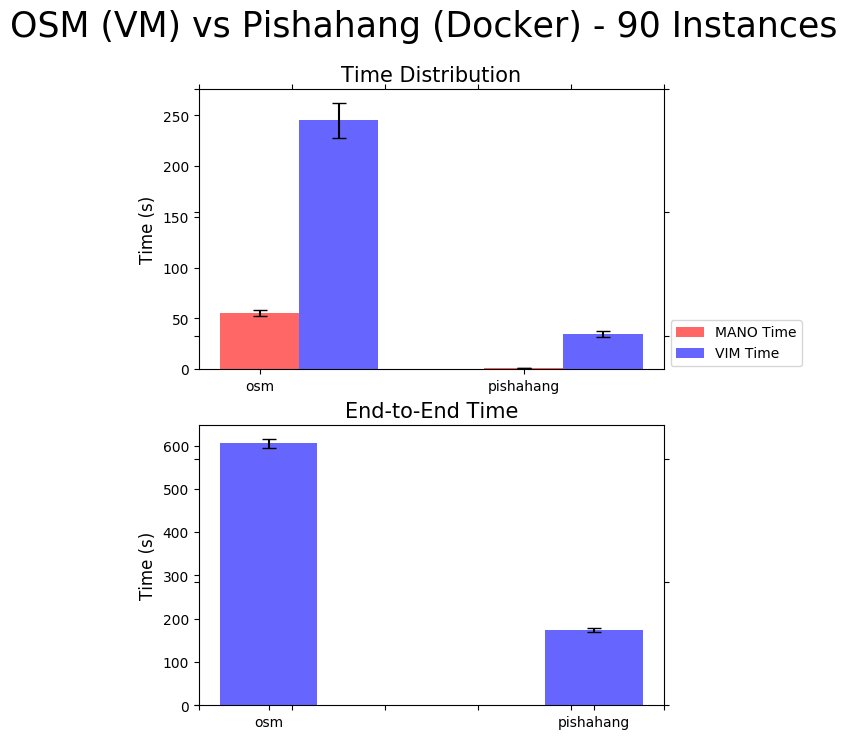
\includegraphics[width=0.7\linewidth]{figures/scalability_graphs/Comparison-VM-Docker/Time_comparison}
	\caption{Time distribution in MANO and VIM}
	\label{fig:timecomparison}
\end{figure}


\begin{figure}[h]
	\centering
	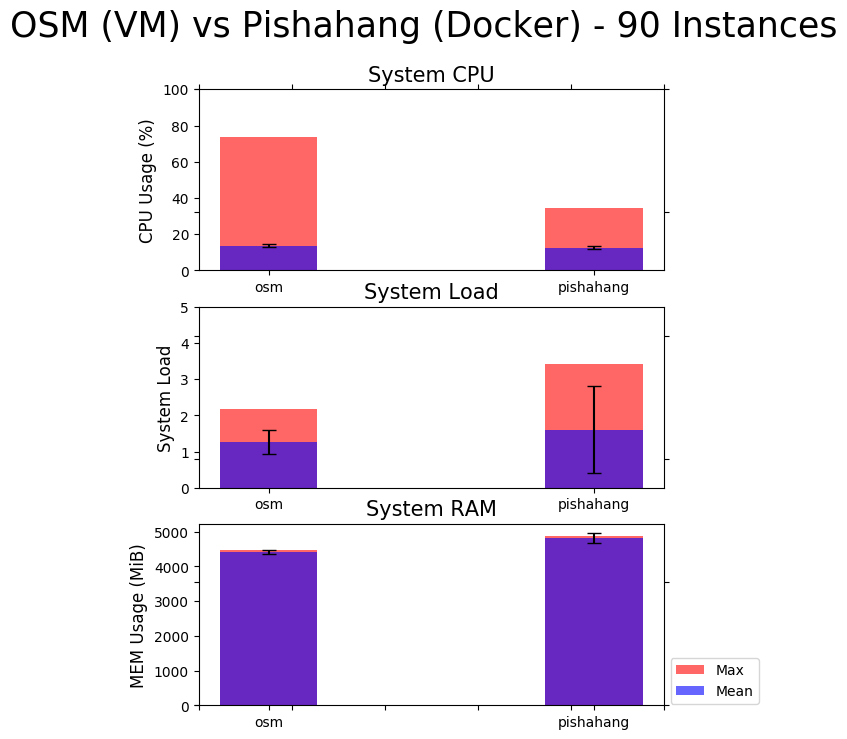
\includegraphics[width=0.7\linewidth]{figures/scalability_graphs/Comparison-VM-Docker/System_metrics_comparison}
	\caption{System resource utilization}
	\label{fig:systemmetricscomparison}
\end{figure}




\subsubsection{Scaling Plugin Evaluation}

We utilized MBF to evaluate our Scaling Plugin discussed in the section \ref{scalingplugin}. 
The Parent Pishahang instance is running the scaling plugin in debug mode, which can be used to mock system load values. 
We added a REST call to the MBF flask server to mock the system load values in the scaling plugin.\\

The experiment was designed to instantiate 90 instances of  cirros docker containers on Pishahang. 
After sending 30 instantiation requests, the experiment script alters the \textit{5m} system load to greater than 0.7, which triggers Rule 1 from the SLP rule set \ref{list:splrules}. 
Thus, creating a new child Pishahang instance. 
However, in the debug mode, for the scope of this experiment, we had a child instance already instantiated from start.\\

After instantiating 45 instances, the script mocks the \textit{15m} system load value to greater than 0.7, which triggers Rule 2 from the SLP rule set \ref{list:splrules}. 
Thus, parent instance will now redirect any further service requests (i.e., 46th instantiation requests on-wards) to the child Pishahang instance.

We use the overall lifecycle data collected by MBF to visualize the CPU usage over time of the top 3 microservices (based on CPU usage).\\

The experiments ran from 11:17:02 to 11:28:23. 
Initially the microservices on the parent instance took all the load, as it can be seen from the figure \ref{fig:parent-top-3-lifecycle}. 
At about the half way mark, the requests are redirected to the child instance. 
The load distributed to the child instance can be seen in the figure \ref{fig:child-top-3-lifecycle}. 


\begin{figure}
	\centering
	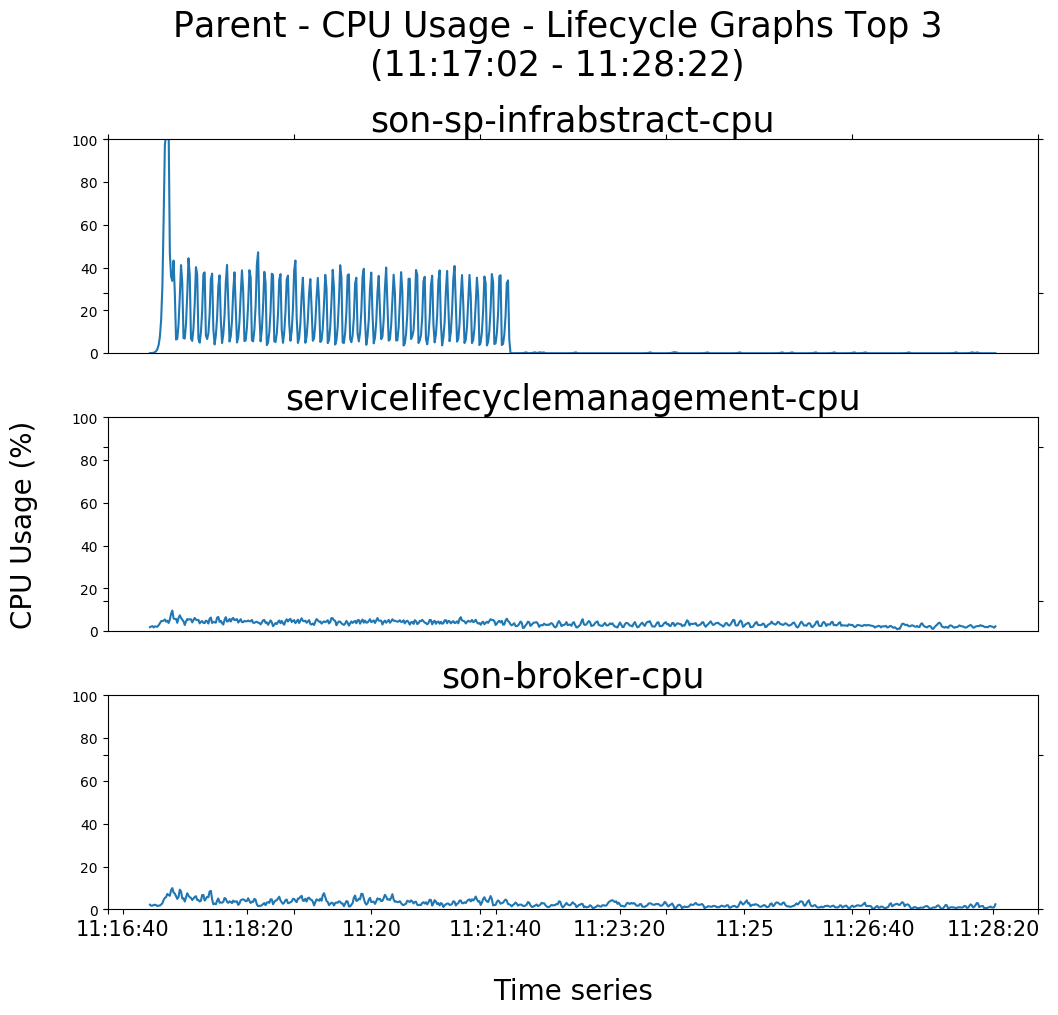
\includegraphics[width=0.65\linewidth]{figures/scalability_graphs/Scalability-Evaluation/Parent-TOP-3-Lifecycle}
	\caption{Parent MANO instance lifecycle graph}
	\label{fig:parent-top-3-lifecycle}
\end{figure}

\begin{figure}
	\centering
	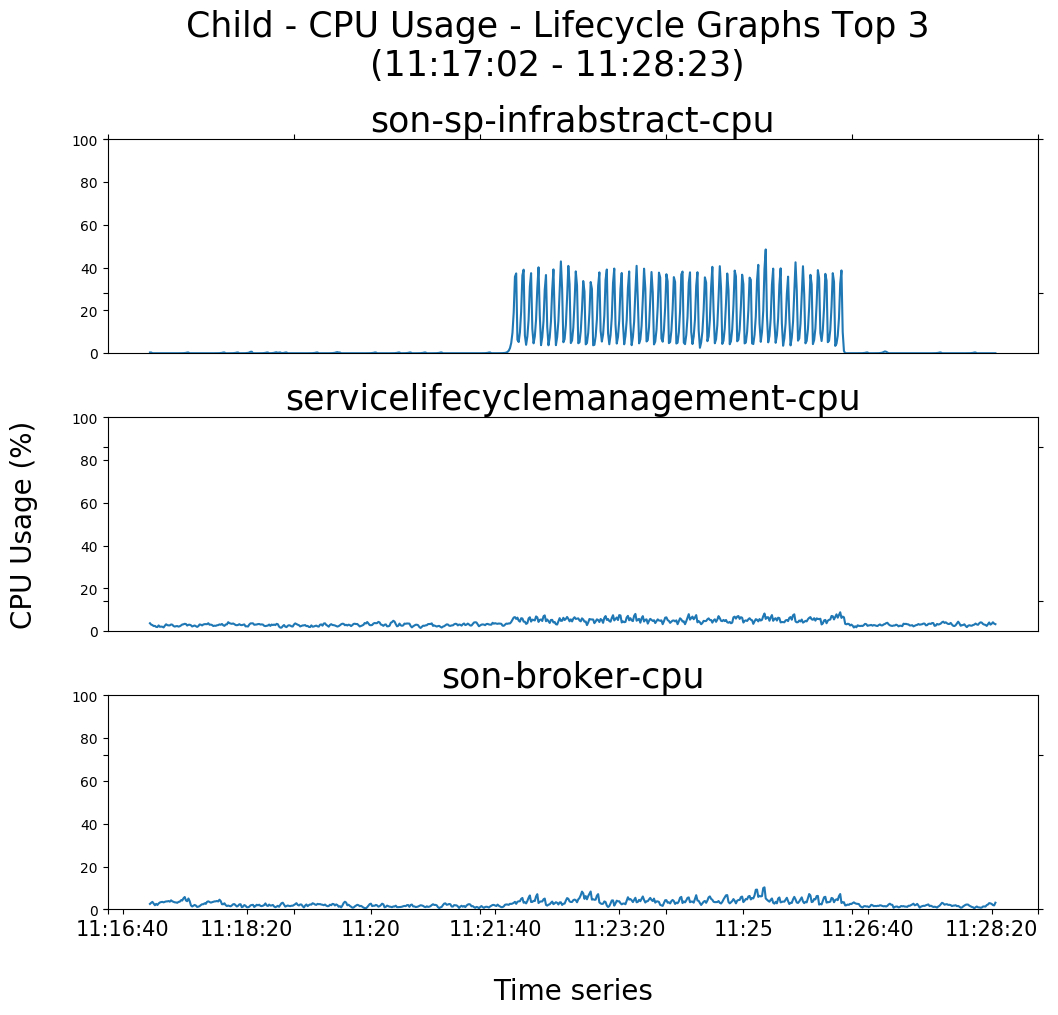
\includegraphics[width=0.65\linewidth]{figures/scalability_graphs/Scalability-Evaluation/Child-TOP-3-Lifecycle}
	\caption{Child MANO instance lifecycle graph}
	\label{fig:child-top-3-lifecycle}
\end{figure}

\pagebreak

\section{Discussions}

In this section, we discuss the observations and inferences drawn from all the experiments conducted on OSM and Pishahang.

\subsubsection{Requests per minute (RPM)}

We observed that the number of successful instantiation of network services and RPM are inversely proportional. For this, we instantiated 90 cirros instances at various RPMs and compared the successful instantiations of VNFs. We carried out this experiment on OSM as the support for VM orchestration is only a proof of concept in Pishahang and we could not instantiate more than 10 instances at once. \\

We saw that when the service requests are sent at 30, 60 and 120 RPMs all the VNFs were successfully instantiated in VIM. But, when the requests where sent at 240 RPMs, we saw on average, 67 successful instantiations, 5 resulted in build errors on the VIM and the remaining requests were lost at the MANO side due to timeouts and internal server errors. \\ 

An interesting observation here is the end-to-end deployment times of various RPMs, i.e, the time taken between the start of instantiation requests and all the instances getting successfully instantiated. We see from the table below that the end-to-end time actually increased with RPM. Even though the requests from the MANO are sent faster, VIM is taking much longer to actually process the requests. \\

\begin{tabular}{|c|c|}
\hline 
\textbf{RPM} & \textbf{End-to-End time}\\ 
\hline 
30 & 555 \\ 
\hline 
60 & 550 \\ 
\hline 
120 & 691 \\ 
\hline 
\end{tabular} 

\subsubsection{NSDs with different number of VNFDs}
To observe the differences in resource utilization for different network services, we designed three different NS. These 3 NS differed in the number of VNFs, i.e, 1, 3 and 5 VNFs respectively.  All the VNFs are cirros images which is used primarily for testing. We also created 3 more identical NS with Ubuntu cloud image as the VNF. The NS are all instantiated in such a way that the number of instantiations remain the same irrespective of the number of VNFs.
For example, if the first NS that has one VNF is instantiated 15 times, the second NS is instantiated five times because it has 3 VNFs. 
The third NS is instantiated three times as it has 5 VNFS, so that all the three NS will result in 15 VNF instantiations on the VIM. 
Similarly, we also had 90 and 180 instantiations.\\

We observed that NS with more number of VNFs consumed more CPU than the ones with lesser number of VNFs. The image type (cirros or Ubuntu) does not make a difference on the resource utilization on the MANO but it does have an effect on the VIM side due to the more physical resources required by the Ubuntu image. \\

Results of the top 2 CPU consuming microservices for OSM are shown in the figure \ref{fig:osmro-mean-cpu-cases} and \ref{fig:osmlcm-mean-cpu-cases}. Results of top 2 CPU consuming microservices for Pishahang are shown in the figure \ref{fig:pishson-mean-cpu-cases} and \ref{fig:pishslm-mean-cpu-cases}

\begin{figure}
\centering
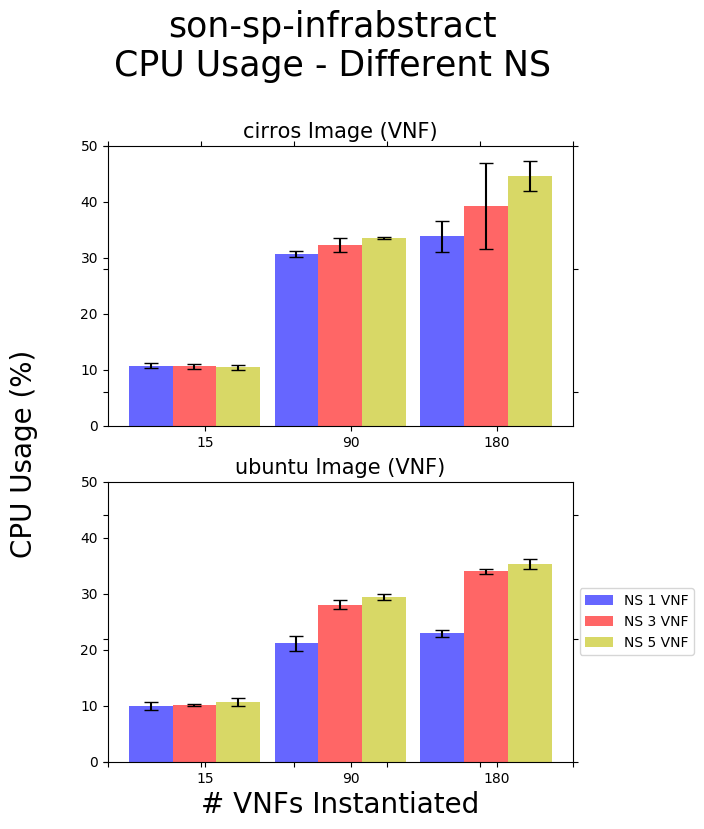
\includegraphics[width=0.7\linewidth]{figures/scalability_graphs/Docker-Grouped-Cases/pishahang/son-sp-infrabstract-cpu-Mean-CPU-Cases}
\caption{CPU usage of Pishahang microservice son-sp-infrabstract}
\label{fig:pishson-mean-cpu-cases}
\end{figure}

\begin{figure}
\centering
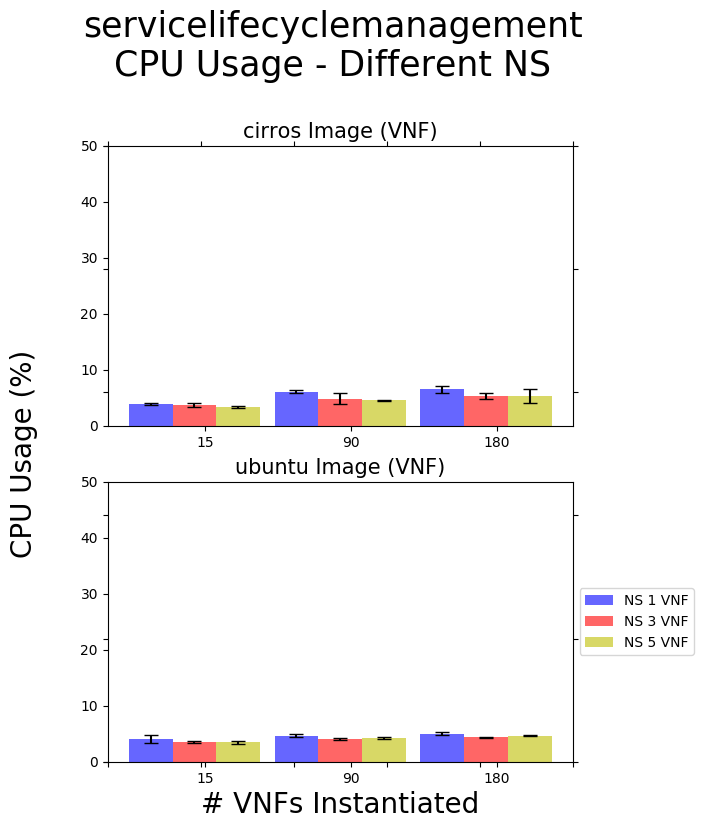
\includegraphics[width=0.7\linewidth]{figures/scalability_graphs/Docker-Grouped-Cases/pishahang/servicelifecyclemanagement-cpu-Mean-CPU-Cases}
\caption{CPU usage of Pishahang microservice servicelifecyclemanagement}
\label{fig:pishslm-mean-cpu-cases}
\end{figure}


\subsubsection{Container v/s VM}

We wanted to compare the resource utilization of two MANO frameworks for orchestration of similar NS. But, Pishahang's support for VM orchestration is unstable. Hence, we were not able to successfully instantiate more than a few (i,e. about 10) NS continuously. It was out of scope of our work to look into the issue and fix them. However, Pishahang has a stable support for container orchestration. We thus decided to compare containers and VMs. The results are discussed in the section \ref{vmvscontainer}.
	
\subsection{Understanding OSM lifecycle graphs}

The figure \ref{fig:osm-top-3-lifecycle-90} shows the lifecycle graphs of the experiment for instantiating 90 instances of the basic cirros NS at 30 RPM. As discussed in the previous sections, the top 3 microservices in terms of CPU usage are RO, LCM and MON respectively.\\

To further understand the uneven peaks and the general trend of RO and LCM graphs, we used a performance profiling tool called Pyflame\footnote{https://github.com/uber/pyflame}. It takes snapshots of the Python call stack to profile a program without modifying its source code. We used Pyflame on the RO and LCM python processes running inside their respective docker containers and started our experiment. We captured flame graphs every 30 seconds and analysed the frequency distribution of the function calls in these containers. This will give us a better understanding of the functionality that is taking the CPU resource. \\

We identified the major function calls of RO and LCM by analyzing the flame graphs. We looked into the source code to understand the functionality and the list containing the references is given below.

\begin{itemize}
\item \textbf{RO Functions}
\begin{itemize}
\item \texttt{\textbf{\_refres\_elements}} \footnote{\url{https://osm.etsi.org/gitweb/?p=osm/RO.git;a=blob;f=osm\_ro/vim\_thread.py;h=d5301f1a6eafa3bf55fe3b4bea17537527dc731d;hb=refs/heads/v5.0\#l253}}

\item \texttt{\textbf{\_proccess\_pending\_tasks}} \footnote{\url{https://osm.etsi.org/gitweb/?p=osm/RO.git;a=blob;f=osm\_ro/vim\_thread.py;h=d5301f1a6eafa3bf55fe3b4bea17537527dc731d;hb=refs/heads/v5.0\#l522}}

\item \texttt{\textbf{new\_vm}} \footnote{\url{https://osm.etsi.org/gitweb/?p=osm/RO.git;a=blob;f=osm\_ro/vim\_thread.py;hb=73ce6ce177937bac038f892e75dfe5a95dc8feeb\#l810}}

\item \texttt{\textbf{del\_vm}} \footnote{\url{https://osm.etsi.org/gitweb/?p=osm/RO.git;a=blob;f=osm\_ro/vim\_thread.py;hb=73ce6ce177937bac038f892e75dfe5a95dc8feeb\#l863}}
\end{itemize}

\item \textbf{LCM Functions}

\begin{itemize}

\item \texttt{\textbf{instantiate}} \footnote{\url{https://osm.etsi.org/gitweb/?p=osm/LCM.git;a=blob;f=osm\_lcm/ns.py;h=83e7147234c66cb348f1c78877fd602781b1b987;hb=refs/heads/v5.0\#l597}}

\item \texttt{\textbf{terminate}}\footnote{\url{https://osm.etsi.org/gitweb/?p=osm/LCM.git;a=blob;f=osm\_lcm/ns.py;h=83e7147234c66cb348f1c78877fd602781b1b987;hb=refs/heads/v5.0\#l1125}}

\item \texttt{\textbf{kafka\_ping}}\footnote{\url{https://osm.etsi.org/gitweb/?p=osm/LCM.git;a=blob;f=osm\_lcm/lcm.py;hb=f609c16f40cef9c60d73c842d858ba457ab3549b\#l190}}
\end{itemize}

\end{itemize}

We plotted the frequency distribution of these functions over experiment time, the resulting graph can be seen in the figure \ref{fig:osm-frequency-dist}. The instantiation requests are coming into OSM until \textit{9:32:54}, by looking at the figure \ref{fig:osm-top-3-lifecycle-90} and \ref{fig:osm-frequency-dist} it can be seen that all the 4 RO functions listed above are active during this period causing the spikes. It is similar in the LCM graph, the \texttt{instantiate} and \texttt{terminate}  functions took the most CPU and the spikes that are seen every 120 seconds in the LCM graph is caused by the \texttt{kafka\_ping} function, which is used to keep the connection to the message broker active. 

When the requests stop coming in, i,e. from \textit{9:32:54}, RO gradually processes all the remaining instantiation tasks and this can be seen from the graphs. 

At \textit{9:38:59}, the termination requests start coming into OSM and a spike in RO and LCM can be seen from the graphs.\\

The MON microservice however, is responsible for continuously monitoring the health of VNFs from the VIMs. We did not profile the MON processes in this experiment.

\begin{figure}[h]
\centering
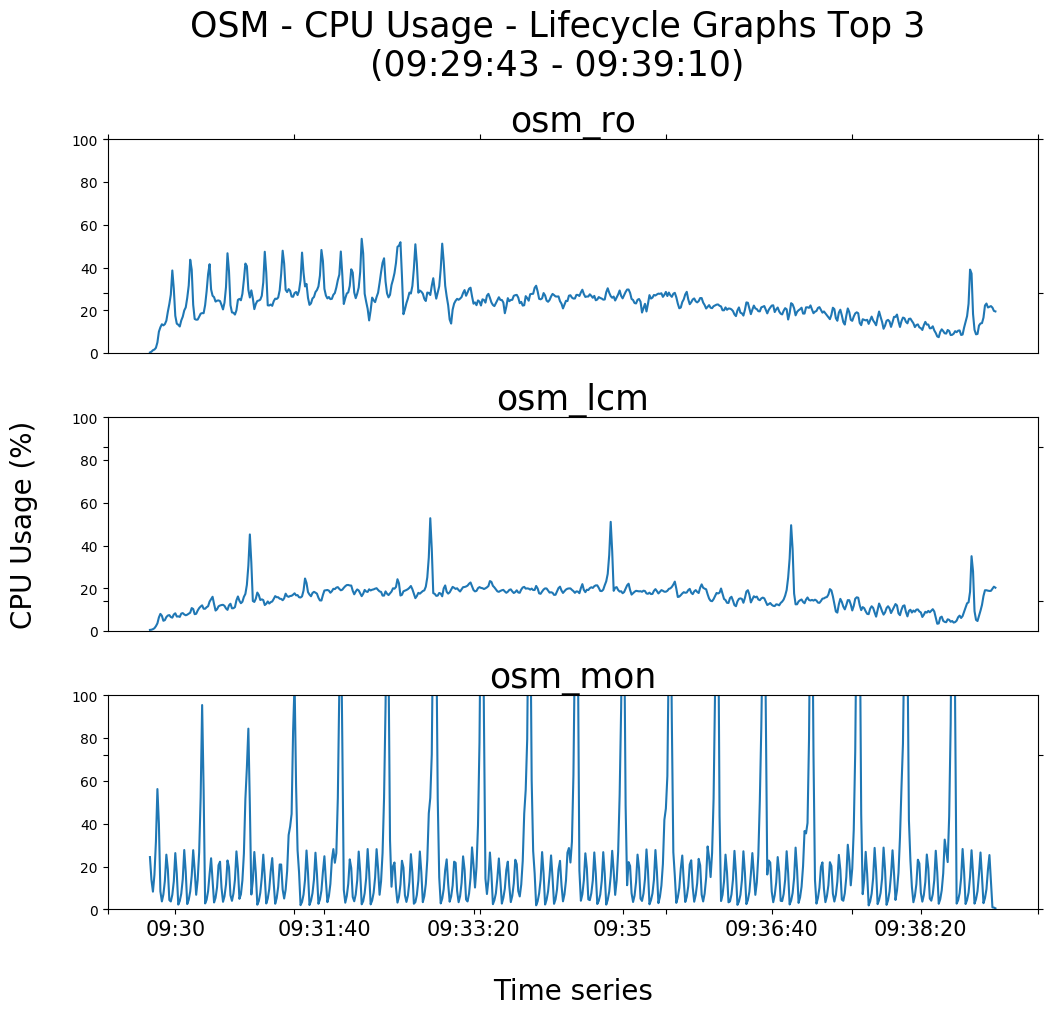
\includegraphics[width=1\linewidth]{figures/scalability_graphs/Lifecycle-Graphs-Top-3/OSM-TOP-3-Lifecycle-90}
\caption{Lifecycle graph for 90 instances}
\label{fig:osm-top-3-lifecycle-90}
\end{figure}

\begin{figure}[h]
\centering
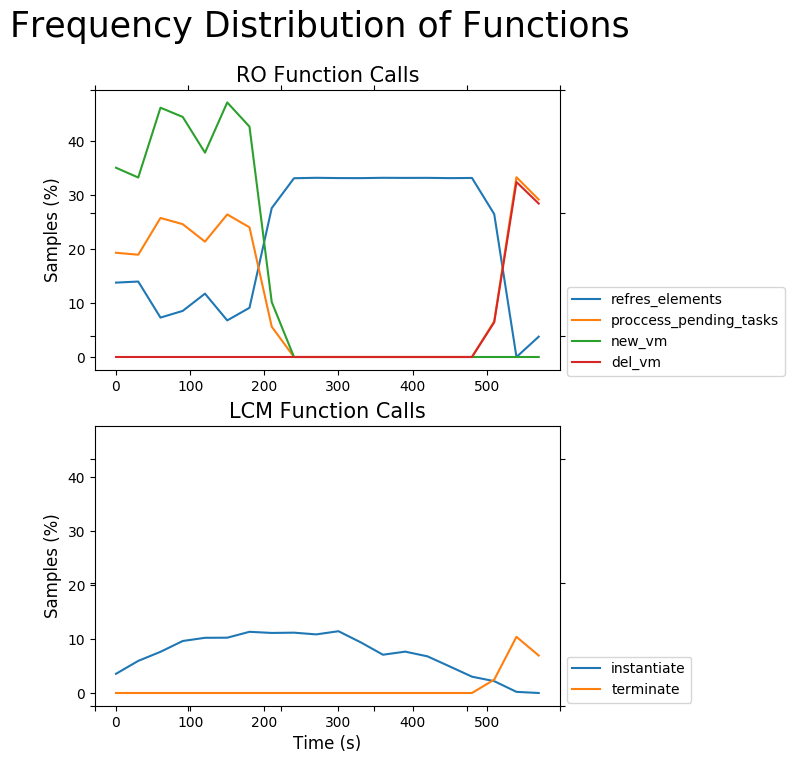
\includegraphics[width=1\linewidth]{figures/scalability_graphs/Lifecycle-Graphs-Top-3/osm-frequency-dist}
\caption{OSM Frequency distribution of functions}
\label{fig:osm-frequency-dist}
\end{figure}
